% Original book p31; original base PDF p35; input PDF p44; p031_s15 四、操作
% Role: answer; original field: diagrams[0].tikz
% Compile with XeLaTeX from this figures/ directory.
\documentclass[12pt,tikz,border=5pt]{standalone}
\usepackage{fontspec}
\setmainfont[Path=../fonts/]{DroidSansFallback.ttf}
\setsansfont[Path=../fonts/]{DroidSansFallback.ttf}
\usepackage{amsmath,amssymb}
\usepackage{tikz}
\usetikzlibrary{calc,angles,quotes,arrows.meta,decorations.pathreplacing,decorations.pathmorphing,decorations.markings,patterns,positioning,fit,backgrounds,matrix,intersections,shapes.geometric}
\begin{document}
\color{red}
\tikzset{every picture/.append style={color=red}}
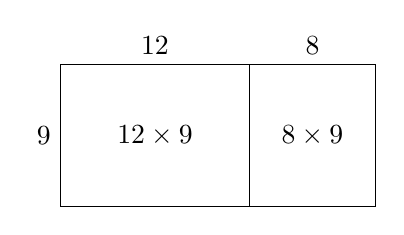
\begin{tikzpicture}[x=.2cm,y=.2cm]\draw(0,0)rectangle(20,9);\draw(12,0)--(12,9);\node[above]at(6,9){12};\node[above]at(16,9){8};\node[left]at(0,4.5){9};\node at(6,4.5){$12\times9$};\node at(16,4.5){$8\times9$};\end{tikzpicture}

\end{document}
